\documentclass{scrreprt}
\usepackage{amsmath}
\usepackage{listings}
\usepackage{array}
\usepackage{tikz} 
\usepackage{underscore}
\usepackage[bookmarks=true]{hyperref}
\usepackage[utf8]{inputenc}
\usepackage[english]{babel}
\usepackage{enumitem}
\usepackage[a4paper, margin=1in]{geometry}
\usetikzlibrary{shapes, arrows.meta, positioning, backgrounds}

% Define styles for different node types
\tikzstyle{startstop} = [rectangle, rounded corners, minimum width=3cm, minimum height=1cm, text centered, draw=black, fill=red!30]
\tikzstyle{process} = [rectangle, minimum width=3.5cm, minimum height=1cm, text centered, draw=black, fill=blue!30]
\tikzstyle{arrow} = [thick,->,>=stealth]

% Define stickman style
\tikzset{
    stickman/.pic={
        % Head
        \draw[fill=gray] (0,0.6) circle (0.3cm);
        % Body
        \draw[line width=0.5mm] (0,0.3) -- (0,-0.6);
        % Arms
        \draw[line width=0.5mm] (-0.4,0.3) -- (0.4,0.3);
        % Legs
        \draw[line width=0.5mm] (0,-0.6) -- (-0.4,-1.2);
        \draw[line width=0.5mm] (0,-0.6) -- (0.4,-1.2);
    }
}

% Hyperref settings
\hypersetup{
    pdftitle={Software Requirement Specification},
    pdfauthor={Jean-Philippe Eisenbarth},
    pdfsubject={TeX and LaTeX},
    pdfkeywords={TeX, LaTeX, graphics, images},
    colorlinks=true,
    linkcolor=blue,
    citecolor=black,
    filecolor=black,
    urlcolor=purple,
    linktoc=page
}

% Set extra row height and padding
\setlength{\extrarowheight}{4pt}
\renewcommand{\arraystretch}{1.5}

\begin{document}

\begin{titlepage}
    \centering
    \includegraphics[width=0.5\textwidth]{./logo.png} 
    \vspace{1cm}

    \textbf{Department of Computer Science and Engineering}\\
    Premier University
    \vspace{1cm}

     \large \textnormal{CSE 302 : Computational Methods for Engineering 
    Problems Laboratory }
    \vspace{1in} 

    \Large \textnormal{Title: Implementation of Bisection, Falsi, and Newton-Raphson Methods for Root Finding}
    \vspace{0.5in} 

    \large
    \textbf{Submitted by:}
    \vspace{0.5cm}

    \renewcommand{\arraystretch}{1.5} 
    \begin{tabular}{|p{0.4\textwidth}|p{0.6\textwidth}|}
        \hline
        \textbf{Name} & Mohammad Hafizur Rahman Sakib \\
        \hline
        \textbf{ID} & 0222210005101118 \\
        \hline
        \textbf{chapter} & C \\
        \hline
        \textbf{Session} & Spring 2024 \\
        \hline
        \textbf{Semester} & 5th Semester \\
        \hline
        \textbf{Submission Date} & 14.09.2024 \\
        \hline
    \end{tabular}
    \vspace{1cm}

    \begin{minipage}[t]{0.48\textwidth}
        \textbf{Submitted to:}\\
        Kollol Dey\\
        Lecturer, Department of EEE\\
        Premier University\\
        Chittagong
    \end{minipage}%
    \hfill
    \begin{minipage}[t]{0.48\textwidth}
        \raggedleft
        \textbf{Remarks}\\
        \vspace{0.5cm} % Adjust vertical space for remarks
        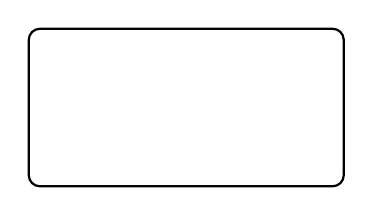
\begin{tikzpicture}
            \draw[thick, rounded corners] (0,0) rectangle (4,2);
        \end{tikzpicture}
    \end{minipage}

    \date{\today}
    \vfill
\end{titlepage}

\section{Introduction}
This report presents the implementation and output of three widely used root-finding methods: the Bisection method, the False Position (Falsi) method, and the Newton-Raphson method. Each method is applied to solve a given mathematical equation, and the code along with its output is provided. The goal is to demonstrate how each algorithm approaches root finding without comparing their efficiencies or convergence rates.

\section{Methods}

\subsection{Bisection Method}
The Bisection method is a simple iterative algorithm for finding roots by repeatedly dividing an interval in half and selecting the subinterval where the root lies. The process is repeated until the interval is sufficiently small.

\subsubsection{Source Code}
\begin{figure}[h]
    \centering
    \includegraphics[width=\textwidth]{path/to/code_image_bisection.png}
    \caption{Bisection Method Source Code}
\end{figure}

\subsubsection{Output}
\begin{figure}[h]
    \centering
    \includegraphics[width=\textwidth]{path/to/output_image_bisection.png}
    \caption{Bisection Method Output}
\end{figure}

\subsection{False Position (Falsi) Method}
The False Position method is similar to the Bisection method but chooses the next interval based on a secant line, which improves the speed of convergence.

\subsubsection{Source Code}
\begin{figure}[h]
    \centering
    \includegraphics[width=\textwidth]{path/to/code_image_falsi.png}
    \caption{False Position Method Source Code}
\end{figure}

\subsubsection{Output}
\begin{figure}[h]
    \centering
    \includegraphics[width=\textwidth]{path/to/output_image_falsi.png}
    \caption{False Position Method Output}
\end{figure}

\subsection{Newton-Raphson Method}
The Newton-Raphson method uses the derivative of the function to find successive approximations to the root. It typically converges faster but requires a good initial guess.

\subsubsection{Source Code}
\begin{figure}[h]
    \centering
    \includegraphics[width=\textwidth]{path/to/code_image_newtonraphson.png}
    \caption{Newton-Raphson Method Source Code}
\end{figure}

\subsubsection{Output}
\begin{figure}[h]
    \centering
    \includegraphics[width=\textwidth]{path/to/output_image_newtonraphson.png}
    \caption{Newton-Raphson Method Output}
\end{figure}

\section{Conclusion}
This report demonstrates the implementation of the Bisection, False Position, and Newton-Raphson methods for solving a root-finding problem. Each method successfully finds the root, and the code and outputs are included to show the process and results. Further analysis could compare the efficiency and convergence behavior of these methods.

\end{document}
